\section{Process and start/end blocks}
The process block, as the name suggests, is responsible for each action. For programming code analysis, this block corresponds to a function call or an assignment operation. The start/end block in this application differs from the process block only in that it signals the starting point and all possible endings of the algorithm in a given scheme. The application automatically replaces the process blocks at the beginning and end with a start/end block. Additionally, the application ignores all $whitespace$ characters. If we want to enter a space character in the diagram block, use the character ``\_'' (underscore), which will be replaced. The application does not force the use of syntax elements implying that it is a function call (ending with ``... ();'') or an assignment (operator ``=''), to draw this block it is only required that only word characters  are used in any language (if having a Unicode equivalent). 
	
	\begin{figure}[H]
  \begin{subfigure}[t]{0.49\textwidth}
    \vspace{0pt}
    \centering
    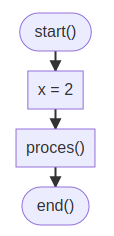
\includegraphics[height=6cm]{proces.png}
  \end{subfigure}\hfill
  \begin{subfigure}[t]{0.49\textwidth}
    \begin{minted}[linenos=true]{cpp}
start();
x _ = _ 2;
proces();
end();
    \end{minted}
  \end{subfigure}%
  \caption{Process, start/end blocks with the code that created those blocks}
\end{figure}

\section{Conditional block }
  \subsection{$if-else$ statement }	 
	
	  The application recognizes the syntax of the statement and creates a decision block for the given condition. Then it creates two branches responsible for actions (any number of process blocks) performed in the event of the condition being met (directly under the scope of the $if$ statement) or not being met (under the scope of the $else$ statement), and then the instructions outside the $if-else$ statement after both branches are being merged.   
		
\begin{figure}[H]
  \begin{subfigure}[t]{0.49\textwidth}
    \vspace{0pt}
    \centering
    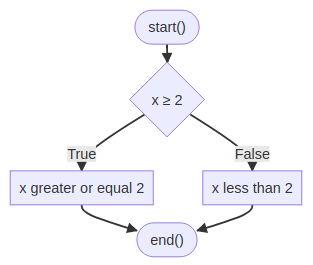
\includegraphics[height=6cm]{decyzja-if-eng.png}
  \end{subfigure}\hfill
  \begin{subfigure}[t]{0.44\textwidth}
    \begin{minted}[xleftmargin=\parindent, linenos=true]{cpp}
start();
if(x _≥ _2){
  x _greater _or _equal _2;
}
else{
  x _less _than _2;
}
end();
    \end{minted}
  \end{subfigure}%
  \caption{Conditional block created with the $if$ statement. Example also shows support for Unicode characters (``≥'' used in this case)}
\end{figure}

		\subsection { $while$ statement } 
	
		The condition interpretation works in the same way as for the $if$ statement, the same applies to adding subsequent statements that are executed after the condition is met, with the difference that the last process of this branch is automatically connected with the decision block of the $while$ statement. Failure to meet the condition corresponds to the branch on which the processes located outside the scope of this type of conditional statement are located.
	
\begin{figure}[H]
  \begin{subfigure}[t]{0.49\textwidth}
    \vspace{0pt}
    \centering
    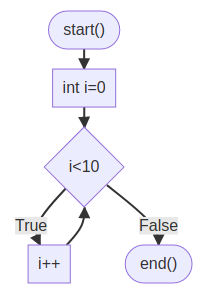
\includegraphics[height=6cm]{decyzja-while.png}
  \end{subfigure}\hfill
  \begin{subfigure}[t]{0.44\textwidth}
    \begin{minted}[linenos=true]{cpp}
start();
int_ i = 0;
while(i < 10){
  i++;
}
end();
    \end{minted}
  \end{subfigure}%
  \caption{Conditional block created with the $while$ statement}
\end{figure}	

\section{More complex example}
Flowchart diagram showing the simplified algorithm of the application in which it was drawn: {\smallskip}

\begin{figure}[H]
  \begin{subfigure}{\textwidth}
    \centering
    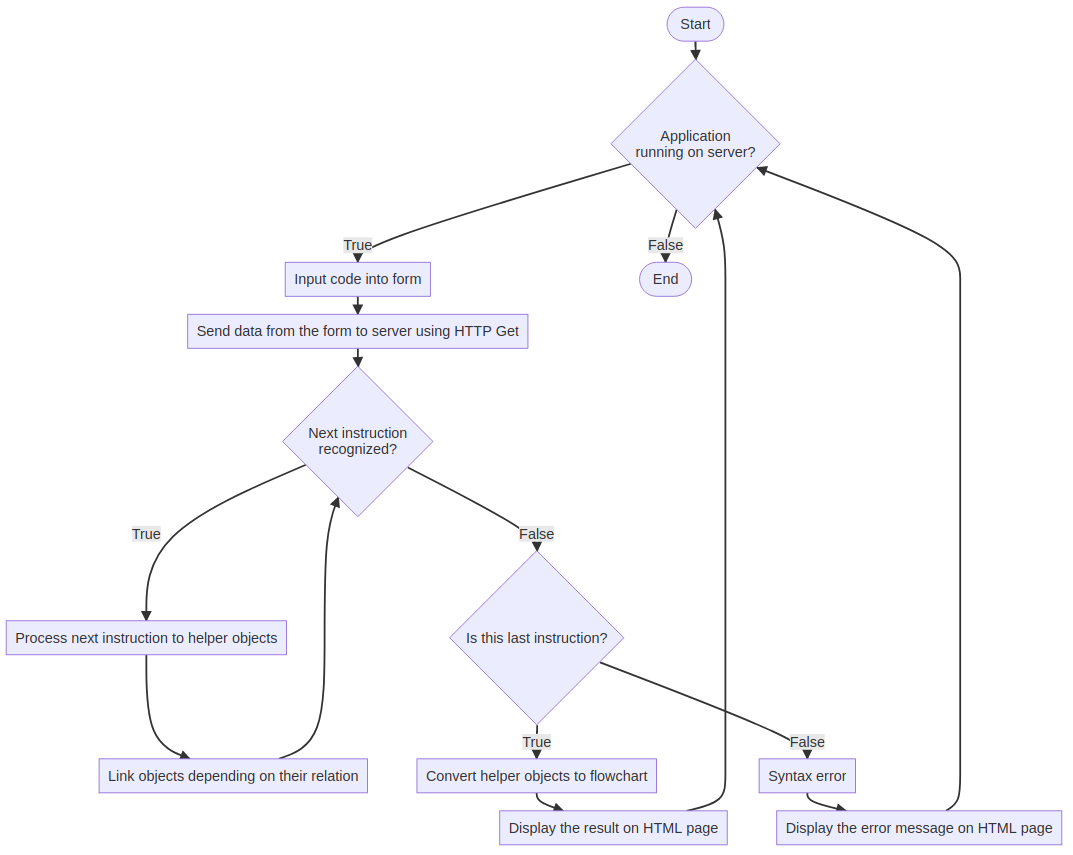
\includegraphics[width=0.97\textwidth]{aplikacja-flowchart-eng.png}
  \end{subfigure}\hfill
  \begin{subfigure}[t]{0.44\textwidth}
    \begin{minted}[linenos=true]{cpp}
Start;
while(Application _running _on _server){
    Input_ code_ into_ form;
    Send _data _from _the _form _to _server _using _HTTP _Get;
    while(Next _instruction _recognized?){
        Process _next _instruction _to _helper _objects;
        Link _objects _depending _on _their _relation;
    }
    if(Is _this _last _instruction?){
    Convert _helper _objects _to _flowchart;
    Display _the _result _on _HTML _page;
    } else {
        Syntax _error;
        Display _the _error _message _on _HTML _page;
    }
}
End;
    \end{minted}
  \end{subfigure}%
  \caption{An example showing handling of nested conditional statements and text wrapping}
\end{figure}